%!TEX ROOT=../diploma-thesis.tex

\chapter{Rešerše}\label{ch:reserse}

V této kapitole se budeme věnovat rešerši existujících řešení
a výzkumu relevantního k tématu této práce. Prozkoumáme
modelem řízenou architekturu, její výhody, nevýhody a vhodnost
použití. Věnovat se budeme také síťovým architekturám umožňujícím
komunikaci služeb v rámci architektury \gls{SOA}.
Dále se zaměříme na aspektově orientované programování
a na něm založený inovativní přístup k návrhu iformačních systémů \gls{ADDA}.
Nakonec prozkoumáme existující nástroje a specializované jazyky pro zápis
byznysových pravidel.

\section{Modelem ř\'{\i}zená architektura}

Modelem řízená architektura (\gls{MDA} z anglického \textit{Model-Driven
Architecture}) se zaměřuje na návrh \gls{IS} pomocí modelů a jejich
následnou transformaci do spustitelného kódu pomocí generativních nástrojů~\cite{soley2000model}.
Autorem specifikací \gls{MDA} je konsorcium Object Modeling Group (\gls{OMG}),
které se zaměřuje na standardizaci modelovacích standardů pro software
a stojí za modelovacím jazykem \gls{UML}, který je de facto globálním standardem
pro vizualizaci statických i dynamických aspektů softwarových systémů.

\gls{MDA} využívá Platform Independent Model (\gls{PIM}),
který popisuje systém pomocí platformově nezávislého \gls{DSL},
typicky pomocí \gls{UML}. Ten je následně převeden do
Platform Specific Model (\gls{PSM}), tedy modelu využívajícího
specifických aspektů platformy, pro kterou má být systém postaven.
Tím může být obecný programovací jazyk či jiné \gls{DSL}.
Nakonec je \gls{PSM} transformován do spustitelného kódu.

Hlavní výhodou \gls{MDA} je vysoká úroveň abstrakce a z toho vyplívající
deduplikace kódu. Pokud je byznysové pravidlo zachyceno v nejvyšší
úrovni modelu, může pak snadno být distribuováno do systému na všechna
místa, kde má být aplikováno. Další výhodou je usnadnění tvorby a zvýšení
kvality kódu díky jeho automatickému generování.

Hlavní nevýhodou \gls{MDA}, která zabraňuje jejímu využití
pro náš účel, je jednosměrný dopředný proces, kterým je výsledný kód z modelu
generován. Pokud dojde ke změně požadavků, je potřeba přegenerovat
celou aplikaci od \gls{PIM} až k finálnímu kódu. Kód, který bylo
nutno doplnit ručně, může snadno zastarat a je potřeba ho manuálně
projít a opravit. Změna byznysových pravidel v našem případě by
navíc při využití \gls{MDA} vyžadovala znovu-nasazení celého
systému, což je v přímém rozporu s požadavkem na možnost dynamicky
upravovat či přidávat byznysová pravidla za běhu systému.

Další nevýhodou tohoto přístupu je jeho závislost na \gls{OOP},
které samotné není schopné se efektivně vypořádat s průřezovými
problémy~\cite{cemus2014aspect}, jak si popíšeme v sekci~\ref{sec:aop}.
Ačkoliv je \gls{MDA} známá již od roku 2000, generativní nástroje pro
její podporu jsou stále nevyspělé a pro některé platformy úplně chybí.

\section{Síťové architektury}

Jak jsme již naznačili v sekci~\ref{sec:soa}, architektura orientovaná na služby staví
na počítačových síťích, díky kterým spolu mohou jednotlivé služby efektivně komunikovat.
Proto je vhodné provést rešerši základních síťových architektur,
abychom mohli co nejlépe navrhnout framework pro centrální správu
a automatickou distribuci byznysových pravidel.

\subsection{Architektura klient-server}\label{sec:client-server}

Model klient-server popisuje vztah mezi komponentami systému, klienty a serverem.
Klient zašle požadavek serveru a ten mu vrátí odpověď~\cite{berson1992client}.
Tento model může být použit obecně i v rámci jednoho počítače,
nejčastěji je však využíván v síťové komunikaci mezi více počítači.
V tomto případě klient sestaví síťové spojení k serveru a po získání odpovědi
od serveru spojení zase uzavře. Schéma komunikace je znázorněno
na obrázku ~\ref{fig:client-server}.

\begin{figure}[t]
    \centering
    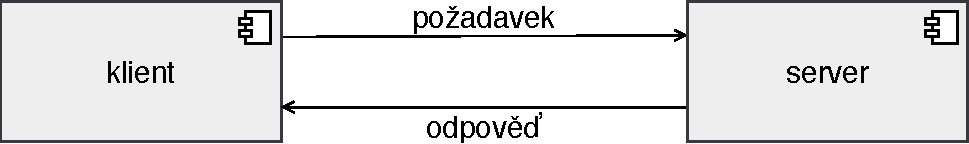
\includegraphics[keepaspectratio=true, width=0.6\linewidth]{figures/client-server.pdf}
    \caption{Architektura klient-server}
    \label{fig:client-server}
\end{figure}

Tato architektura je jednou ze základních stavebních kamenů
internetových protokolů. Využívá ji zejména protokol
\gls{TCP}~\cite{postel1981transmission}, který je hlavním
komunikačním protokolem v síti Internet. Jako příklad si můžeme představit
prohlížení internetových stránek. Uživatel zadá \gls{URL} adresu
stránky, kterou chce navštívit, a internetový prohlížeč, potažmo uživatelův osobní počítač,
v roli klienta odešle požadavek na server nacházející se na dané adrese.
Server požadavek přijme, zpracuje, a odešle odpověď obsahující
tělo webové stránky. Klient stránku přijme a zobrazí pro koncového
uživatele.

Tento přístup má několik zásadních výhod, díky kterým se stal
široce využívaným. Díky svojí velmi obecné myšlence je nezávislý
na jakékoliv platformě a jako klient i server mohou sloužit
jak vysoce výkonné počítače, tak i osobní počítače nebo chytré telefony,
z nichž každý může využívat odlišné operační systémy –
stačí aby klient i server uměl komunikovat stejným protokolem.
Zároveň tato architektura přesouvá byznysovou logiku a
ukládání dat na server a díky tomu umožňuje
snadnější kontrolu nad systémem a jeho centrální administraci. S tím
je spojena i snažší škálovatelnost systému. V neposlední řadě
přináší model klient-server díky centralizaci i lepší zabezpečení,
kdy server může jasně definovat a vynucovat přístupová pravidla.

Hlavní nevýhodu této architektury je vytvoření jednoho centrálního bodu,
jehož výpadek ochromí funkci celého systému (v angličtině
\textit{single point of failure}) \textendash\xspace tímto bodem je server.
Pokud na serveru nastane chyba či výpadek, žádný z klientů není schopen využívat
jeho služeb.

Pro sdílení byznysových pravidel se tato architektura jeví
jako vhodná. Klient, který potřebuje byznysové pravidlo ke
svém funkci, by zažádal server o dané pravidlo a po jeho získání by
se postaral o jeho spuštění. Tím by bylo dosaženo automatické
distribuce a integrace byznysových pravidel. Vzhledem k tomu,
že server je v této architetkuře centrální autoritou, usnadnila
by se tak centrální správa byznysových pravidel.

\subsection{Architektura Peer-to-peer}\label{sec:p2p}

Opakem modelu klient-server je síťová architektura zvaná \textit{Peer-to-peer (\gls{P2P})}.
Jednotlivé počítače v síti spolu komunikují přímo, bez centrální autority.
Všechny počítače v síti jsou si vzájemně rovnocenné.~\cite{fox2001peer}
Na obrázku~\ref{fig:peer-to-peer} je tato architektura znázorněna.
Hlavním cílem \gls{P2P} sítí je distribuce dat nebo výpočetních operací.

\begin{figure}[t]
    \centering
    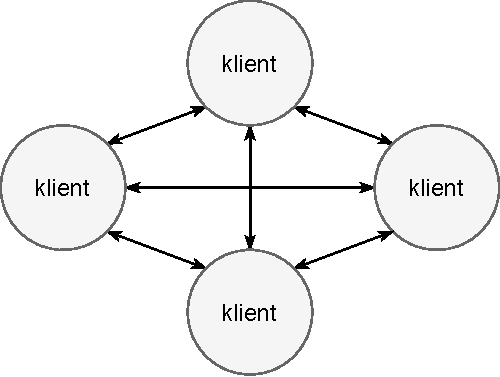
\includegraphics[keepaspectratio=true, width=0.4\linewidth]{figures/peer-to-peer.pdf}
    \caption{Architektura peer-to-peer}
    \label{fig:peer-to-peer}
\end{figure}

Jednotliví klienti mezi sebou zpravidla vytvářejí virtuální síť, tzv. \textit{overlay},
která je postavená nad fyzickou sítí, přes kterou jsou reálně fyzicky zasílány zprávy mezi klienty.
Typicky je tato virtuální síť podmnožinou existující fyzické sítě. Výhodou tohoto přístupu je,
že klienti jsou abstrahováni od fyzického uspořádání počítačů a mohou spolu komunikovat napřímo,
i když mezi nimi mohou reálně být v síti zapojeny jiné počítače.

Nespornou výhodou architektury \gls{P2P} je, že s rostoucím počtem klientů roste i
kapacita a výkon sítě, narozdíl od modelu klient-server, kdy se klienti musí dělit o výkon serveru.
Navíc v takové síti neexistuje \textit{single point of failure} a tak se zvyšuje její robustnost.

Mezi silné nevýhody této architektury patří zvýšená bezpečnostní rizika způsobená tím,
že klienti jsou otevřeni komunikaci s jakýmkoliv jiným, potenciálně nebezpečným, klientem.
Potenciální útočník tak může velmi snadno využít zranitelností na dálku.
Další hrozbou je to, že některý z klientů může \textit{otrávit} síť
(z anglického \textit{network poisoning}) podvrženými daty, která jsou pak
nekontrolovatelně šířena mezi všechny klienty. Z toho vyplývající nevýhodou
může být absence jakékoliv centrální správy sdílených dat.

Ačkoliv se může \gls{P2P} jevit jako vhodný přístup pro sdílení byznysových pravidel
díky svojí orientaci na sdílení dat, vysoké datové propustnosti a robustnosti, právě absence
centrální správy by mohla uvrhnout systém do nekonzistentního stavu při úpravě či přidání
byznysového pravidla. Tato architektura totiž implikuje, že by byznysové pravidlo bylo
replikováno a distribuováno mezi více uzlů sítě. Změna pravidla by se tak musela šířit postupně
napříč systémem, přičemž některé uzly by stále využívaly starou verzi pravidla, a nad samotným
šířením by neměl administrátor systému kontrolu.

\subsection{Representational state transfer}\label{sec:rest}

Representational state transfer~\cite{fielding2000rest} (\gls{REST}) je architektura
webových služeb, která staví na protokolu \gls{HTTP}, a klade na systém
několik architektonických omezení, díky kterým může systém dosáhnout
lepšího výkonu, vyšší škálovatelnosti, jednoduchému používání díky jednotnému rozhraní
a lepší odolnosti vůči chybám. V roce 2000 ho ve své dizertační práci představil Roy Fielding,
který je zároveň hlavním autorem specifikace \gls{HTTP} 1.1~\cite{fielding1999hypertext}.

\gls{REST} chápe data systému jako množinu zdrojů (z anglického \textit{resources}),
nad kterými jsou prováděny operace pomocí \gls{HTTP} požadavků. K odlišení operací
nad jedním zdrojem jsou využívána slovesa protokolu \gls{HTTP}, zejména pak \code{GET} pro čtení,
\code{POST} pro vytváření, \code{PUT} pro úpravu a \code{DELETE} pro mazání. Tím jsou zastřešeny
všechny \gls{CRUD} operace.

\begin{figure}[t]
    \centering
    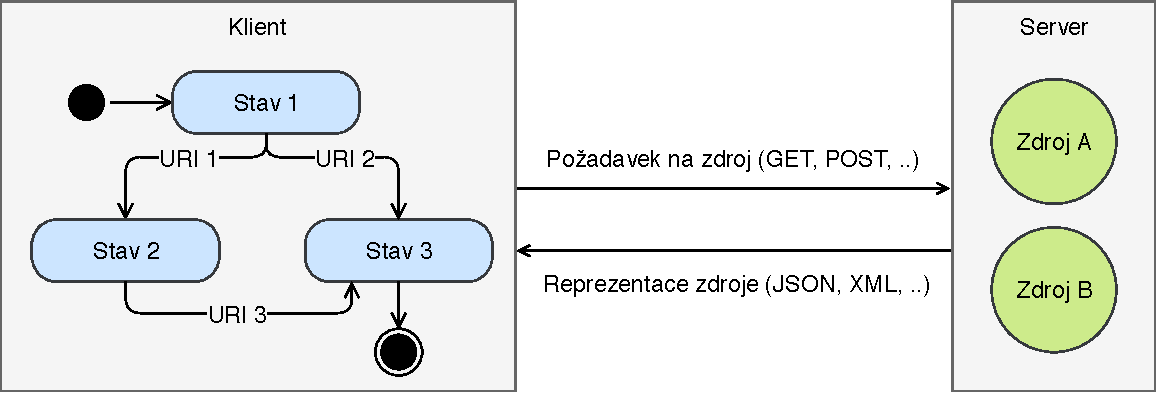
\includegraphics[keepaspectratio=true, width=0.9\linewidth]{figures/rest-statelessness.pdf}
    \caption{Znázornění architektury \gls{REST}}
    \label{fig:rest-statelessness}
\end{figure}

Principy architektury \gls{REST} jsou:

\begin{description}
    \item [Klient-server] Systém by měl využívat model klient-server. Díky tomu může jasně oddělit
    zodpovědnost za uživatelské rozhraní na klienta a zodpovědnost za ukládání dat na server. To zvyšuje
    škálovatelnost systému díky nižším nárokům na server.
    \item [Bezstavovost] Každý požadavek na server by měl obsahovat všechny informace potřebné k jeho vykonání.
    Kromě těla \gls{HTTP} požadavku se k tomuto účelu často využívají i hlavičky požadavku,
    například hlavička \code{Authorization} pro autentizaci uživatele kvůli přístupu k zabezpečeným zdrojům.
    Tím se zjednodušuje komplexita serveru, který plně přesouvá zodpovědnost za uchování stavu uživatelského rozhraní
    na klienta, jak je znázorněno na obrázku~\ref{fig:rest-statelessness}. Nutno poznamenat, že stav dat v systému
    je stále uchováván na serveru.
    \item [Kešování] Odpovědi serveru musí obsahovat explicitní informaci o tom, zda lze odpověď uložit do cache.
    Díky tomu je možné znovupoužívat data, která již server jednou vrátil, a jejich životnost má dlouhodobější charakter.
    Tím se zvyšuje výkon celého systému.
    \item [Vrstvený systém] Klient by neměl mít možnost rozeznat, zda komunikuje přímo se serverem, nebo s prostředníkem,
    např. s proxy serverem, load balancerem nebo cache.
    \item [Code-on-demand] Volitelným požadavkem na systém je tzv. \textit{code-on-demand}, který umožňuje serveru vracet
    spustitelný kód jako odpověď. Klient kód poté spustí na své straně. Typickým příkladem jsou klientské JavaScriptové aplikace spouštěné ve webových prohlížečích.
    \item [Jednotné rozhraní] Zdroje systému musejí mít unikátní identifikátor, např. \gls{URI}. Zdroje jsou při komunikaci reprezentovány libovolným formátem, který
    se může lišit od interní reprezentace zdroje v programu, např. \gls{JSON} či \gls{XML}. Reprezentace zdroje musí být
    dostatečná k tomu, aby šlo na zdroji provést úpravu či smazání. Zprávy mezi klientem a serverem musejí obsahovat veškerá potřebná metadata,
    aby druhá strana mohla zprávu plně zpracovat. K tomu se používají například \gls{HTTP} hlavičky \code{Content-type}
    či \code{Accept}, ve kterých je popsán typ reprezentace zdroje.
    Rozhraní by také mělo dodržovat koncept \textit{Hypermedia as the engine ot application state (\gls{HATEOAS})},
    který vyžaduje, aby server v odpovědích vracel metainformace o struktuře jeho \gls{API}.
    Klient je tak schopen dynamicky navigovat v rozhraní serveru aniž by bylo vyžadováno předem znát přesné adresy zdrojů.
    Princip \gls{HATEOAS} se však ve většině reálných \gls{API} zanedbává či implementuje pouze částečně.
\end{description}

Nevýhody architektury \gls{REST} spočívají zejména v náročnosti její korektní implementace,
která se v praxi často zjednodušuje, a tím jsou degradovány její výhody. Přes rošířenost a popularitu
této architektury ji stále mnoho vývojářů nezná do detailu a zanedbává některé její části.
Většina programovacích jazyků je založena na volání funkcí či metod, což svádí vývojáře ke
špatnému návrhu systému. \gls{REST} totiž naopak vyžaduje od vývojáře nad systémem přemýšlet jako
nad množinou zdrojů. Jinou nespornou nevýhodou je náročná implementace transakcí, které zahrnují více
zdrojů najednou. Protokol \gls{HTTP} nepodporuje uzavření více požadavků do jedné atomické
transakce. To může být problém v \gls{SOA} zejména pokud je vyžadována kooperace více služeb
najednou při vykonávání byznysové operace. Existují však koncepty, které využívají model
Try-Cancel/Confirm~\cite{pardon2011towards}, umožňující zajistit atomické transakce nad \gls{REST} architekturou.
Jak jsme již zmínili v sekci~\ref{sec:microservices}, moderní systémy se přiklánějí ke konceptu
\textit{eventual consistency}, kdy jsou tolerovány drobné nekonzistence, které jsou nakonec
dořešeny manuálně, pokud je cena za ně menší než cena za implementaci systému, který
by plně podporoval atomické transakce.

\subsection{Remote procedure call}\label{sec:rpc}

Remote procedure call (\gls{RPC}) je podstatně starší architekturou než \gls{REST}.
Tento termín byl použit již v roce 1981 Brucem Nelsonem~\cite{nelson1981remote}.
Architektura staví na modelu klient-server a její princip je velmi jednoduchý \textendash\xspace
umožňuje jednomu procesu, klientovi, zavolat proceduru na druhém, vzdáleném procesu, tedy serveru.
Klient zašle serveru zprávu vyžadující zavolání specifické procedury. Server
proceduru provede a po jejím dokončení zašle klientovi odpověď s návratovou hodnotou.
Klient poté může pokračovat ve své práci.

Zásadním bodem je fakt, že \gls{RPC} kompletně obstarává komunikaci, a v programu samotném
je vzdálená procedura volána stejným způsobem jako lokální procedury. Základním
prvkem architektury na klientovi i na serveru je tzv. \textit{stub}, tedy komponenta, která
umožňuje volat, resp. obsloužit, vzdálenou proceduru lokálně a zapozdřuje veškerou síťovou komunikaci
a serializaci či deserializaci argumentů, resp. návratových hodnot. Schéma komunikace
je znázorněno na obrázku~\ref{fig:rpc}.

\begin{figure}[t]
    \centering
    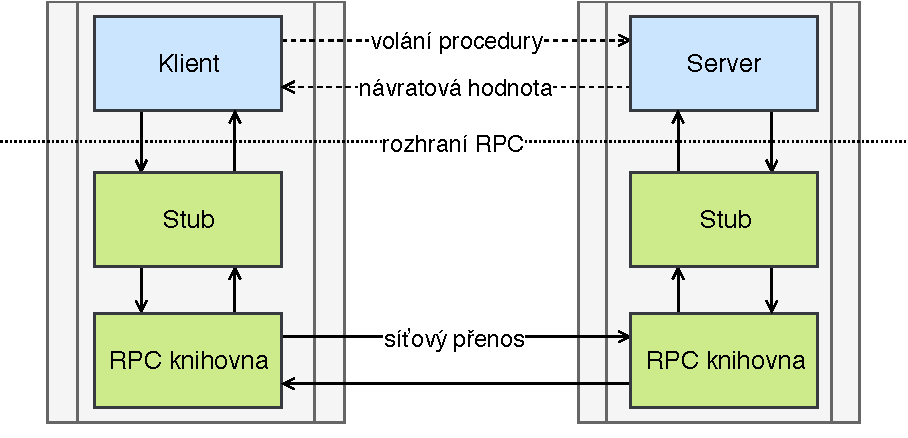
\includegraphics[keepaspectratio=true, width=0.7\linewidth]{figures/rpc.pdf}
    \caption{Schéma komunikace \gls{RPC}}
    \label{fig:rpc}
\end{figure}

Představitelem architektury \gls{RPC} je například technologie \gls{CORBA},
kterou jsme již popsali v sekci~\ref{sec:corba}, nebo technologie Remote Method Invocation (\gls{RMI})
v jazyce Java. Modernějším pojetím je technologie gRPC~\cite{grpcio}
od společnosti Google\footnote{https://www.google.com/},
která je v dnešní době hojně využívána úspěšnými technologickými společnostmi.

Již zmiňovanou nevýhodou abstrakce lokálních a vzdálených volání jsou
negativní vlastnosti síťové komunikace, tedy její zvýšená latence
a nižší robustnost. Pokud programátor nemá možnost zjistit, zda volá
lokální či vzdálenou proceduru, výsledný kód může být těžké optimalizovat
a správně ošetřit výjimky, které mohou při jeho běhu nastat.

Na druhou stranu, narozdíl od \gls{REST} není pro \gls{RPC} potřeba
implementovat komplexní middleware obstarávající síťovou komunikaci,
serializaci a zpracování chyb. Middleware je zpravidla dodáván v podobě knihoven
dané technologie. Exsitují příklady funkcionality, která může být mnohem přirozeněji
realizována pomocí volání procedur, než jako entita reprezentující systémový zdroj.

Vhodnost \gls{RPC} architektury pro distribuci a správu byznysových pravidel je do značné
míry ovlivněna tím, jakou konkrétní technologii využijeme. Stejně jako \gls{REST}
ani \gls{RPC} nedefinuje jakým způsobem by měly být obslouženy transakce. Byli bychom tedy
nuceni si transakční systém doimplementovat. To by však mohlo být o něco snažší díky tomu,
že by obsluha transakce mohla být volána jako procedura, a tím bychom si ušetřili práci
s obslužným kódem.

\section{Aspektově orientované programován\'{\i}}\label{sec:aop}

\subsection{Motivace}

\goal{Co je paradigma}
Programován\'{\i} je komplexn\'{\i} discipl\'{\i}na s teoreticky
neomezen\'ym počtem možnost\'{\i}, jak\'ym programátor může
řešit zadan\'y problém. Ačkoliv každá úloha má své specifické
požadavky, za relativně krátkou historii programován\'{\i} se
stihlo ustálit několik ideologi\'{\i}, tzv. programovac\'{\i}ch
paradigmat, které programátorovi poskytuj\'{\i} sadu abstrakc\'{\i}
a základn\'{\i}ch principů~\cite{van2009programming}.
D\'{\i}ky znalosti paradigmatu může programátor nejen zlepšit
svou produktivitu, ale zároveň může snáze pochopit myšlenky
jiného programátora a t\'{\i}m zlepšit kvalitu t\'ymové spolupráce.

\goal{OOP a jeho popis}
Jedn\'{\i}m z nejpopulárnějš\'{\i}ch paradigmat použ\'{\i}van\'ych k
v\'yvoji modern\'{\i}ch enterprise systémů je nepochybně
objektově orientované programován\'{\i} (\gls{OOP}). To vn\'{\i}má dan\'y problém
jako množinu objektu, které spolu intereaguj\'{\i}. Program
člen\'{\i} na malé funkčn\'{\i} celky odpov\'{\i}daj\'{\i}c\'{\i} struktuře
reálného světa~\cite{rentsch1982object}. Je vhodné zm\'{\i}nit,
že objekty se rozum\'{\i} jak konkrétn\'{\i} koncepty, např\'{\i}klad
auto nebo člověk, tak i abstraktn\'{\i} koncepty,
namátkou bankovn\'{\i} transakce nebo objednávka v obchodě.
Objekty se pak prom\'{\i}taj\'{\i} do kódu programu i do
reprezentace struktur v paměti poč\'{\i}tače.
Tento př\'{\i}stup je velmi snadn\'y pro pochopen\'{\i},
vede k lepš\'{\i}mu návrhu a organizaci programu a snižuje
tak náklady na jeho v\'yvoj a údržbu.

\goal{Nedostatky OOP}
Ačkoliv je \gls{OOP} velmi siln\'ym a všestrann\'ym nástrojem,
existuj\'{\i} problémy, které nelze s jeho pomoc\'{\i} efektivně řešit.
Jedn\'{\i}m takov\'ym problémem jsou obecné požadavky na systém,
které musej\'{\i} b\'yt konzistentně dodržovány na v\'{\i}ce
m\'{\i}stech systému, které spolu zdánlivě nesouvis\'{\i}.
Takové požadavky naz\'yváme \textit{průřezové problémy}
(z anglického \textit{cross-cutting concerns}).
V rámci \gls{OOP} je programátor nucen v ojektech manuálně opakovat
kód, kter\'y zodpov\'{\i}dá za jejich realizaci. Duplikace kódu
vede k větš\'{\i} náchylnosti na lidskou chybu a k vyšš\'{\i}m nárokům na v\'yvoj
a údržbu daného softwarového systému~\cite{fowler1999refactoring}.
Obrázek~\ref{fig:cross-cutting} znázorňuje vzájemné postavení průřezových
problémů a komponent informačního systému.

\begin{figure}[t]
    \centering
    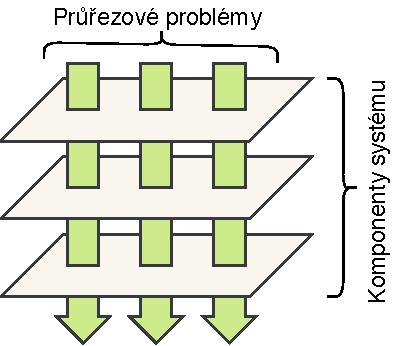
\includegraphics[keepaspectratio=true, width=0.35\linewidth]{figures/cross-cutting.pdf}
    \caption{Průřezové problémy v informačních systémech}
    \label{fig:cross-cutting}
\end{figure}

\goal{Konkrétní příklad nedostatku OOP}
Př\'{\i}kladem průřezového problému může b\'yt logován\'{\i}
systémov\'ych akc\'{\i}, optimalizace správy paměti
nebo jednotné zpracován\'{\i} v\'yjimek~\cite{kiczales1997aspect},
ale i aplikace byznysových pravidel~\cite{cemus2014aspect}.
Uvážme e-commerce systém a zpracování transakcí. To musí
být zohledněno jak při vytváření objednávek, tak při registraci
nového uživatele \textendash\xspace dvě byznysové akce, které by měly
být podle \gls{OOP} implementovány v naprosto odlišných objektech
a striktně odděleny, ale část jejich funkcionality je identická,
a tudíž dochází k duplikaci kódu.

Ve zdrojovém kódu~\ref{lst:tangling} můžeme vidět, jak průřezové
problémy zasahují do kódu imaginární třídy implementované v
jazyce Java, která slouží pro vytváření objednávek v e-commerce
systému popsaném v sekci~\ref{sec:shortcomings}.
Můžeme si všimnout, že aspekt logování je zohledněn na třech
místech, stejně jako aspekt transakcí. Navíc jsou zde zohledněna
i byznysová pravidla pro validaci doručovací a fakturační adresy
objednávky.

\lstinputlisting[
caption={Příklad průřezových problémů zohledněných při vytváření objednávky},
label={lst:tangling},
language=Java,
%frame=single,
float,
floatplacement=t
]
{code/tangling.java}

\goal{AOP jako odpověď na nedostatky OOP}
Aspektově orientované programován\'{\i} (\gls{AOP}) přináš\'{\i} řešen\'{\i} na
v\'yše zmiňované problémy. Extrahuje obecné požadavky,
tzv. \textit{aspekty} do jednoho m\'{\i}sta a pomoc\'{\i} procesu zvaného
\textit{weaving} je poté automaticky distribuuje do systému.
Weaving může proběhnout staticky při kompilaci programu nebo dynamicky
při jeho běhu. V obou př\'{\i}padech ale programátorovi ulehčuje práci,
protože k definici i změně aspektu docház\'{\i} centrálně a t\'{\i}m je eliminována
potřeba manuáln\'{\i} duplikace kódu. Je nutno poznamenat, že \gls{AOP} nen\'{\i}
paradigmatem poskytuj\'{\i}c\'{\i}m kompletn\'{\i} framework pro návrh programu.
V ideáln\'{\i}m př\'{\i}padě je tedy k návrhu systému využita kombinace
\gls{AOP} s jin\'ym paradigmatem. Pro účely této práce se zaměř\'{\i}me na
kombinaci \gls{AOP} a \gls{OOP}.

\subsection{Názvosloví}

\paragraph{Aspekt}
Jak jsme již naznačili, základním pojmem v rámci \gls{AOP} je \textit{aspekt},
který zapozdřuje průřezovou funkcionalitu a zároveň adresuje místa, kde má být
funkcionalita aplikována. Aspekt vždy obsahuje alespoň jeden \textit{advice}
a jeden \textit{pointcut}.

\paragraph{Join-point}
Místo v kódu, na které může být aplikována funkcionalita aspektu, se nazývá
\textit{join-point}. Typů join-pointů je více a závisí na použitém paradigmatu,
na který je \gls{AOP} aplikováno, a také na programovacím jazyce. V případě
kombinace s \gls{OOP} a klasickým víceúčelovým jazykem jako je například Java,
mohou jako join-pointy sloužit konstruktory tříd, volání metod, zápis a čtení
z atributu objektu, inicializace třídy nebo objektu a mnoho dalších.

\paragraph{Pointcut}
Ne každý aspekt je aplikován na každý join-point. Množina join-pointů,
na které je jeden konkrétní aspekt aplikován, se nazývá \textit{pointcut}.
Tato množina může být určena staticky, a být tak známá při kompilaci programu, nebo
dynamicky za běhu programu, což přináší výpočetní složitost navíc.
Dynamické určení pointcutu ale umožňuje vývojářům postihnout i případy,
kdy nelze předem jasně určit místa, kde má být aspekt začleněn.
Příkladem může být zpracování transakcí v zanořených byznysových operacích,
kdy transakce má být započata pouze při vstupu do vnější operace
a dokončena pouze při výstupu z vnější operace.

\paragraph{Advice}
Funkcionalita, kterou aspekt přidává v jeho pointcutu, se nazývá
\textit{advice}. Existuje více typů advice, podle toho, kam je
daná funkcionalita přidána. Například při volání metody může
být funkcionalita přidána před, za, nebo kolem metody.

\paragraph{Weaving}
Proces, kterým jsou advice začleňovány podle pointcutu do
jednotlivých join-pointů se nazývá \textit{weaving}. Ten může
probíhat již při kompilaci nebo dynamicky za běhu programu,
tzv. \textit{run-time weaving}. Proces weavingu je ilustrován
na obrázku~\ref{fig:aspect-weaving}. Komponenta zodpovědná za
weaving se nazývá \textit{aspect weaver}.

\begin{figure}[t]
    \centering
    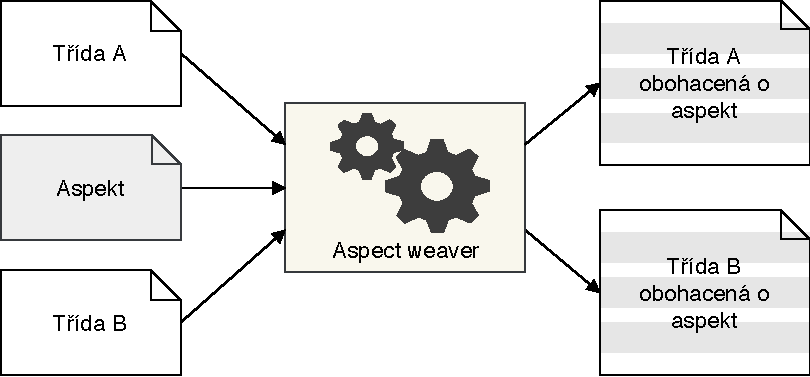
\includegraphics[keepaspectratio=true, width=0.7\linewidth]{figures/aspect-weaving.pdf}
    \caption{Proces weavingu aspektů}
    \label{fig:aspect-weaving}
\end{figure}

\section{Aspect-driven Design Approach}

Alternativním způsobem návrhu informačních systémů, který staví na principech \gls{AOP},
je Aspect-driven Design Approach\footnote{Autoři nejprve používali termín \textit{Aspect-Oriented
Design Approach} (AODA), který byla později změněn. Oba tyto pojmy jsou vzájemně zaměnitelné.}
(\gls{ADDA})~\cite{cemus2014aspect}, představený Karlem Čemusem v roce 2014.
Tento přístup se zaměřuje na formalizaci jednotlivých komponent informačních systémů identifikování aspektů
v informačních systémech a jejich separaci do jednoho bodu, tzv. \textit{single focal point}.
Následně přístup využívá weaving pro automatickou distribuci aspektů do systému.
K popisu aspektu doporučuje využití doménově specifického jazyka, který bude navržen na
míru danému průřezovému problému.

\subsection{Možnosti aplikace}

Autoři \gls{ADDA} aplikovali tento koncept v několika oblastech \gls{IS}.
Mezi tyto oblasti patří automatické začleňování byznysových pravidel
do datové vrstvy informačních systémů~\cite{cemus2015automated}, automatické
generování uživatelských rozhraní citlivých na kontext uživatele~\cite{cemus2017separation},
validaci vstupů formulářů v uživatelském rozhraní vůči byznysovým pravidlům~\cite{cemus2016context}\cite{cemus2017separation}
a automatické extrakci dokumentace~\cite{cemus2017automated}.

\paragraph{Automatické začleňování byznysových pravidel do datové vrstvy}

Jednou z možných aplikací přístupu \gls{ADDA} je automatické začleňování
byznysových pravidel do datové vrstvy \gls{IS}\footnote{Předpokládáme standardní
třívrstvou architekturu informačních systémů~\cite{fowler2002patterns}}.
Byznysová pravidla jsou nejprve vhodně popsána pomocí \gls{DSL} a následně jsou
extrahována do jednoho bodu, ze kterého jsou automaticky distribuována.
Pomocí specializovaného weaveru jsou pravidla překládána do podmínek
jazyka \gls{JPQL}, potažmo \gls{SQL}, který je využíván k získávání dat
z databázových systémů. To vede ke snížení manuální duplikace byznysových
pravidel.

\paragraph{Automatické generování uživatelského rozhraní}

Uživatelská rozhraní tvoří až 48 \% kódu informačních systému
a zabírají až 50 \% jejich vývojového času~\cite{kennard2009separation}.
Do \gls{UI} se přitom typicky promítá mnoho aspektů, které jsou
již v systému obsaženy, a vývojáři je musí manuálně duplikovat.
Typickým příkladem je struktura datového modelu, která se promítá
zejmána do struktury formulářů sloužících pro manipulaci s daty systému.
Byznysová pravidla jsou promítána do \gls{UI} při validaci vstupních
dat formulářů na straně klienta~\cite{cemus2017separation}.
Dalšími příklady může být lokalizace \gls{UI} do různých jazyků
nebo rozložení a stylizace jednolivých ovládacích prvků, která
je zpravidla uniformní v celém systému.

Autoři přístupu \gls{ADDA} přicházejí s řešením v podobě
využití několika \gls{DSL} pro popis jednotlivých aspektů
a run-time weavingu, který aspekty při běhu aplikace
dynamicky začlení do \gls{UI} s ohledem na aktuální kontext
uživatele, například na jeho geolokační polohu či velikost
displeje, na kterém je rozhraní zobrazováno.
Díky tomu je dosaženo významné redukce kódu~\cite{cemus2016context}
potřebného pro popis adaptibilního uživatelského rozhraní
a tím jsou ušetřeny náklady na vývoj a údržbu informačního
systému využívajícího tento přístup.

\paragraph{Automatická extrakce dokumentace}

Další oblastí informačních systému, do které se promítají jeho aspekty,
je jeho dokumentace~\cite{cemus2017automated}. Autoři \gls{ADDA}
využívají data mining pro získání metainformací o byznysových operacích,
datovém modelu systému a o byznysových pravidlech. Díky tomu mohou
automaticky vygenerovat seznam byznysových operací, potažmo implementovaných
use-cases, strukturu doménového modelu a formální popis byznysových pravidel,
který může sloužit pro verifikaci jejich správnosti.

\subsection{Výhody a nevýhody}

Jak můžeme pozorovat z uvedených příkladů, \gls{ADDA} poskytuje
vývojářům způsob jakým výrazně snížit náklady na vývoj a údržbu
systému díky deduplikaci, která je dosažena extrakcí aspektů
do \textit{single focal point} a jejich automatickou distribucí do
příslušných komponent systému.

Je nutno poznamenat, že tento přístup má svoje úskalí v podobě
vysoké počáteční investice, kterou vyžaduje vývoj specializovaných
\gls{DSL} a dynamických aspect weaverů. Ačkoliv autoři
tohoto přístupu implementovali prototypy knihoven umožňující
požadovanou funkcionalitu, pro nasazení do reálného systému
nejsou tyto knihovny připraveny.

Pro náš účel se však jeví přístup \gls{ADDA} jako vysoce vhodný, protože
rezonuje s cíly této práce. Přístup navíc splňuje požadavky
identifikované v sekci~\ref{sec:implementation-requirements},
zejména využití speciálních \gls{DSL} pro popis aspektů a
jejich automatickou distribuci za běhu systému. Pro popis byznysových pravidel
využívá \gls{ADDA} nástroj \textit{Drools}, který prozkoumáme v následující sekci.

\section{Stávaj\'{\i}c\'{\i} řešen\'{\i} reprezentace business pravidel}\label{sec:business-rule-dsl}

V rámci této kapitoly se zaměřujeme i na současné možnosti zachycení
byznysových pravidel ve specializovaných jazycích a vhodnost jejich použití
pro účel frameworku, který bude výstupem této práce.

Ačkoliv existuje relativně velké množství knihoven poskytujících
\gls{DSL} pro popis byznysových pravidel a umožňující automatickou
distribuci byznys pravidel, žádný z nich neposkytuje podporu velkého
množství programovacích jazyků, resp. platforem, ve kterých by mohl
být jazyk použit. Namátkou můžeme zmínit projekt \textit{business-ruless}
pro jazyk Python~\cite{businessrulespython}, projekt FlexRule pro platformy .NET a
JavaScript nebo \gls{BRMS} JRules~\cite{jrules} od společnosti IBM pro
platformu \gls{Java EE}.

V této sekci se tedy zaměříme zejména na framework Drools, který
používají autoři přístupu \gls{ADDA}, a také na moderní nástroj
JetBrains MPS, který umožňuje vytvářet \gls{DSL} a transformovat je
do libovolných víceúčelových jazyků.

\subsection{Drools DSL}

Framework Drools~\cite{drools} vyvijený společností JBoss\footnote{http://www.jboss.org/}
je open-source projekt realizující \textit{business rule management engine} (\gls{BRMS}),
tedy nástroj pro vývoj a správu byznysových pravidel. Framework umožňuje realizovat
tzv. \textit{produkční systémy}, tedy systémy tvořené sadou \textit{produkčních pravidel}
určujících chování programu. Tato pravidla obsahují popis situace a její řešení v případě,
že nastane. Tyto systémy tedy poskytují určitou formu umělé inteligence, která simuluje
rozhodování experta na danou doménu.

Produkční pravidlo se skládá z levé strany (\gls{LHS} z anglického \textit{left-hand side}),
a z pravé strany (\gls{RHS} z anglického \textit{right-hand side}),
\gls{LHS} popisuje situaci, při které má být pravidlo aplikováno. \gls{RHS} popisuje akci,
která má být vykonána.

Pro správnou funkci systému je nutno při vyhodnocování správně určit, která produkční pravidla
mají být aplikována. Pro tento účel využívá framework Drools algoritmus RETE~\cite{forgy1988rete},
vynalezený Charlesem Forgym v roce 1983, který je přímo navržený pro párování pravidel produkčních systémů.
Využívá stromové paměťové struktury, která minimalizuje výpočetní složitost na úkor paměťové složitosti. Framework
Drools navíc implementuje některá vylepšení algoritmu optimalizující jeho paměťovou složitost.

Součástí frameworku Drools je speciální doménově specifický jazyk vyvinutý přímo
pro modelování produkčních pravidel. Tento jazyk umožňuje popsat \gls{LHS} i \gls{RHS}
daného pravidla a k tomu využívá několik užitečných konstruktů. Pro popis situací i důsledků
využívá dialekt MVEL umožňující komfortní zápis logických výrazů. V rámci Drools \gls{DSL}
lze využívat lokální i globální proměnné s plnou typovou podporu pramenící z jazyka Java a také
podporu regulárních výrazů. Navíc je možno importovat i pomocné funkce, které lze
využít v podmínkách pravidla.

Ve zdrojovém kódu~\ref{lst:drools-example} můžeme vidět příklad zápisu
byznysového pravidla v jazyce Drools DSL. Kromě názvu pravidla je v hlavičce
uvedeno, které dialekty jsou v pravidle využity. Dialekt \code{mvel} jsme již popsali výše a
dialekt \code{java} nám umožňuje pro \gls{RHS} využít přímo jazyk Java. Popsané produkční pravidlo
vypíše uživatelovo jméno a email, pokud má uživatel email vyplněný.

\lstinputlisting[
caption={Ukázka zápisu byznysového pravidla v jazyce Drools DSL},
label={lst:drools-example},
language=Drools,
%frame=single,
float,
floatplacement=t
]
{code/drools_example.drl}

Ačkoliv je jazyk Drools \gls{DSL} vymodelovaný přímo pro zápis pravidel doménovými experty,
odlišnost produkčních pravidel a byznysových pravidel tak, jak jsme si je zavedli v sekci~\ref{sec:business-rules},
je na první pohled zřejmá. Pro naše účely bychom využili pouze \gls{LHS}, protože nám stačí
popsat nastalou situaci, ale o následnou akci se postará systém \textendash\xspace v případě
neúspěšné validace precondition je probíhající byznysová operace zastavena, v případě post-condition je aplikován filtr
na všechny proměnné splňující danou podmínku. Zároveň jazyk Drools \gls{DSL} postrádá
nástroje pro kvalitní popis byznysového kontextu držícího byznysová pravidla,
zejména pak rozšiřování jiných kontextů a popis typu jednotlivých pravidel~\cite{cemus2017automated}.
V neposlední řadě nejsou ze strany frameworku Drools podporovány jiné platformy než
Java a .NET, což nevyhovuje našim požadavkům na platformovou nezávislost.

\subsection{JetBrains MPS}

Zajímavým nástrojem z dílny společnosti JetBrains\footnote{https://www.jetbrains.com/}
je tzv. \textit{MPS \textendash\xspace Meta Programming System}~\cite{jetbrainsmps}, který si klade za úkol být univerzálním
nástrojem pro tvorbu doménově specifických jazyků. Staví na konceptu \textit{language-oriented
programming} (\gls{LOP})~\cite{ward1994language} zaměřujícího se na vývoj velmi specifického jazyka,
který je následně použit pro implementaci programu namísto obecného mnohoúčelového jazyka. Pro překlad
ze specifického jazyka do spustitelného kódu je použit automatický překladač. Příkladem jazyka, který využívá koncept \gls{LOP}
je \LaTeX\xspace, který byl využit pro sazbu této diplomové práce. Ten totiž pomocí maker jazyka \TeX\xspace
sestavuje abstraktnější jazyk, který umožňuje autorovi soustředit se hlavně na strukturu textu, aniž by
se musel příliš detailně zaobírat samotnou sazbou.

MPS umožňuje uživateli nadefinovat gramatiku speciálního \gls{DSL} a následně poskytuje
editor pro tento jazyk včetně validace. MPS podporuje také transformování kódu napsaného
v nadefinovaném jazyce do jiných, nízkoúrovňovějších jazyků, zejména pak do jazyka Java.
Díky tomu lze nejen vytvářet libovolné \gls{DSL}, ale také rozšiřovat existující
jazyky \textendash\xspace například přidat do jazyka Java podporu pro jednoduchý vizuální
zápis matic, jak můžeme vidět na obrázku~\ref{fig:java-matrix}.

\begin{figure}[t]
    \centering
    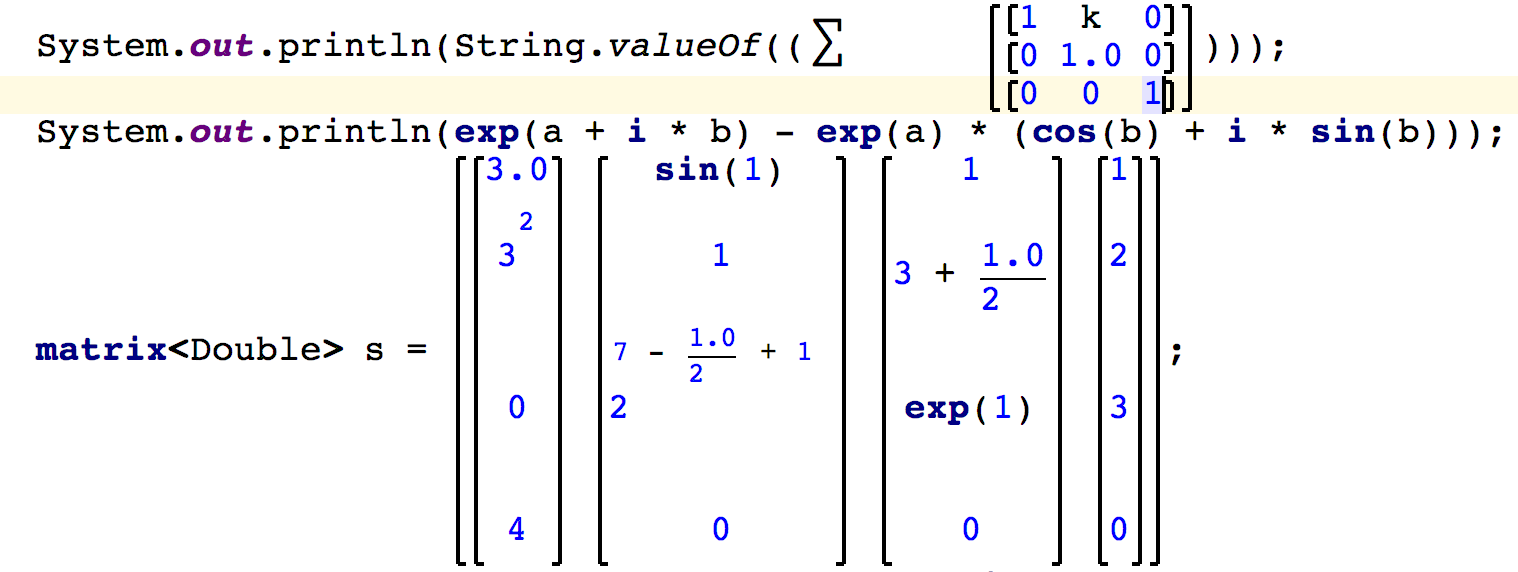
\includegraphics[keepaspectratio=true, width=0.7\linewidth]{figures/java-matrix.png}
    \caption{Rozšíření jazyka java o zápis matic pomocí JetBrains MPS~\cite{jetbrainsmps}}
    \label{fig:java-matrix}
\end{figure}

Výhoda tohoto přístupu je podobně jako u \gls{MDA} vysoká úroveň abstrakce, která
velmi dobře odděluje problém návrhu systému od implementačních problémů.
Navíc lze díky použití \gls{DSL} zapojit do vývoje doménové experty a snížit tak
zátěž na programátory, kteří se mohou více věnovat právě implementačním problémům.
\gls{DSL} typicky zvyšuje expresivitu kódu a díky tomu se zmenšuje jeho objem.
Nižší objem kódu vede ke snížení nákladů na jeho údržbu a vývoj~\cite{littman1987mental}\cite{soloway1986empirical}.
Významnou výhodou MPS, potažmo \gls{LOP}, je vysoká portabilita vyvinutého jazyka.
Pro migraci na jinou platformu stačí doprogramovat překladač jazyka, ale
samotný jazyk může zůstat zachovaný.

Z výčtu výhod plyne, že bychom mohli MPS využít k popisu byznysových pravidel,
resp. byznysových kontextů. Tím bychom získali silný aparát k zachycení a
znovupoužití pravidel a jejich transformaci do neomezeného počtu jazyků pro
využití na mnoha platformách. Podobně jako u \gls{MDA} je však problém v dopředném
generování \textendash\xspace pro případ úpravy pravidla za běhu programu bychom museli
nějakým způsobem upravované pravidlo přetransformovat z dané platformy zpět
do našeho \gls{DSL}, upravit ho pomocí editoru MPS, a následně ho opět přeložit
do spustitelného jazyka pro danou platformu. To by vyžadovalo potřebu překompilovat
a znovu nasadit všechny služby využívající dané pravidlo.

\section{Shrnut\'{\i}}

V této kapitole jsme provedli rešerši \textit{modelem řízené architektury},
jej\'{\i}ch v\'yhod a nev\'yhod. Prozkoumali jsme síťové architektury,
které mohou být využity pro komunikaci služeb v architektuře \gls{SOA}
a zvážili vhodnost jejich použití pro účely této práce.
Shrnuli jsme paradigma \textit{aspektově orientovaného programován\'{\i}} a
věnovali se inovativnímu přístupu k návrhu softwarov\'ych systémů \textit{ADDA}.
Nakonec jsme provedli rešerši stávaj\'{\i}c\'{\i}ch řešen\'{\i} reprezentace byznys pravidel
včetně komplexn\'{\i}ho frameworku \textit{Drools} a zhodnotili jsme jeho vhodnost
k řešen\'{\i} našeho problému.
